\centering
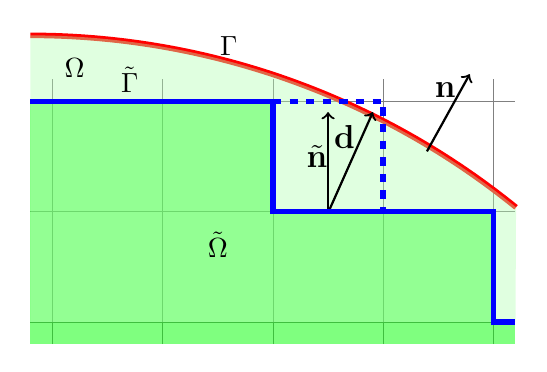
\begin{tikzpicture}[scale=1.4]
    % Draw the Cartesian grid
    \draw[step=1cm, gray, very thin] (0.8,-0.2) grid (5.2,2.2);

    % Highlight cells inside the domain (interior cells)
    \foreach \x/\y in {2/1, 1/0, 1/1, 2/0, 3/0, 4/0}
        {
            \fill[green, opacity=0.5] (\x,\y) rectangle (\x+1,\y+1);
        }
    \foreach \x/\y in {1/0 }{
            \fill[green, opacity=0.5] (\x,\y) rectangle (\x-0.2,\y+2);
        }

    \fill[green, opacity=0.5] (0.8,-0.2) rectangle (5.2,0);

    \draw[line width=2pt, red, domain=51:90, samples=100, variable=\t]
    plot ({0.8 + 7.0*cos(\t)}, {-4.4 + 7.0*sin(\t)});
    \node at (2.6,2.5) {$\Gamma$};

    % Fill the area below the red line with light green to indicate the domain Omega
    \fill[green!30, opacity=0.4] plot[domain=51:90, samples=100, variable=\t] ({0.8 + 7.0*cos(\t)}, {-4.4 +
            7.0*sin(\t)}) -- (0.8,0) -- (5.2,0) -- cycle;

    % Define the angle parameter
    \pgfmathsetmacro{\myangle}{66}
    % Draw a vector from the surrogate boundary to the true boundary
    \draw[<-, thick] ({0.8 + 6.9*cos(\myangle) + 0.3}, {-4.4 + 6.9*sin(\myangle)}) -- ({0.8 + 5.9*cos(\myangle)
            +
            0.3}, {-4.4 +
            5.9*sin(\myangle)});
    % Position the label relative to the vector angle
    \pgfmathsetmacro{\labelangle}{\myangle - 6} % Adjust angle slightly for label placement
    \node at ({0.8 + 6.9*cos(\labelangle) - 0.6}, {-4.4 + 6.9*sin(\labelangle)+0.1}) {\large $\mathbf{d}$};

    \draw[->, thick] ({0.8 + 6.8*cos(\myangle-5) + 0.3}, {-4.4 + 6.8*sin(\myangle-5)}) -- ({0.8 +
            7.6*cos(\myangle-5)
            +
            0.3}, {-4.4 +
            7.6*sin(\myangle-5)});
    \node at ({0.8 + 7.5*cos(\labelangle-5) - 0.54}, {-4.4 + 7.5*sin(\labelangle-5)+0.36}) {\large $\mathbf{n}$};

    % Draw the vector d vertically from the surrogate boundary to the true boundary
    \draw[<-, thick]  ({0.8 + 5.9*cos(\myangle) +
            0.3}, {-4.4 + 6.9*sin(\myangle)}) -- ({0.8 + 5.9*cos(\myangle) +
            0.3}, {-4.4 +
            5.9*sin(\myangle)});
    \node at (3.4, 1.5) {\large $\tilde{\mathbf{n}}$}; % Place label near the normal vector

    % Draw the surrogate boundary (only the top boundary of the interior cells)
    \draw[line width=2pt, blue] (0.8,2) -- (3,2) -- (3,1) -- (4,1) -- (5,1)-- (5,0)-- (5.2,0.) ;

    \draw[line width=2pt, blue, dashed] (3,2) -- (4,2) -- (4,2) -- (4,1) ;
    \node at (1.7,2.2) {$\tilde{\Gamma}$};

    \node at (2.5,0.7) {$\tilde{\Omega}$};

    \node at (1.2,2.3) {${\Omega}$};

\end{tikzpicture}
